\documentclass[a4paper,12pt]{article}
\parindent 1cm
\parskip 1mm
\usepackage{amsmath}
\usepackage[dvips]{epsfig}

\begin{document}

\begin{center}

{\Large\bf CN 530 - Computational Models of Vision}

\bigskip

{\large\bf Assignment \# 4}
\vspace{0.1mm}

\end{center}

{\bf Abstract}
\smallskip

In this assignment we are replicating the phenomena of apparent motion. We will be using our distant dependent shunting network, augmented by a difference-of-gaussians kernel that replicates the on-center off-surround effect of excitatory/inhibitory neurons. 
\smallskip

The phenomena of apparent motion is defined as thus: a stimuli has apparent motion if, given two stimuli flashed at different times at different points in the receptive field, the two will appear as ``connected'', or as the same object moving with respect to time. An example of this you may have seen is in those arcade games with the ring of light bulbs wherein you must press the button when the bulb in front of you illuminates. The lit bulbs appear to form a moving circle because of the temporal and spatial proximity at which they illuminate. Essentially, if one thing flashes nearby and soon after the previous thing, the two things will appear as one moving object. 
\smallskip

This can be replicated in our distant-dependent shunting model by controlling several parameters as we will see in the subsequent sections. Choosing these parameters depends on the properties of your network; apparent motion is possible for any two stimuli, but a practical model should adhere to the realistic properties of distance and SOA between stimuli. 
\vfil\eject

{\bf The Model}
\smallskip

We will use the distant-dependent shunting network of size $n=100$ neurons. The network uses the following equation 

\begin{equation}
\frac{dx_i}{dt}=-Ax_i+(B-x_i) \sum_{k=1}^nI_kC_{ki}-(D+x_i) \sum_{k=1}^nI_kE_{ki}
\end{equation}

to model response, where $C_{ki}$ and $E_{ki}$ represent our excitatory and inhibitory gaussian kernels, respectively. 

\begin{equation}
C_{ki}=Ce^{-\mu(k-i)^2}
\end{equation}
\begin{equation}
E_{ki}=Ee^{-\nu(k-i)^2}
\end{equation}
\bigskip

{\bf The stimuli}
\smallskip

The stimuli presented to our model will simulate two ``flashes'' at different locations and different points in time. The stimuli will occur at locations $k$ and $l$, where $1<k<l<n$. The first stimuli will start at the beginning of the simulation ($t=0$) and the second will start after some stimulus-onset-asynchrony ($t=SOA$). These stimuli will persist for some duration $m$. 
\vfil\eject

{\bf Getting apparent motion}
\smallskip

Given the model and the stimuli, we must control our parameters in order to simulate apparent motion. There are a lot of parameters to play with, and many different combinations will do this for us. 
\smallskip

The plot below represents the two gaussian kernels as well as their difference. The difference curve contains a positive region and a negative region, and these regions spread out over some space. The amount of space covered represents how many neigboring cells fall into the on-center portion and the off-surround portion. 

\begin{center}
  \begin{figure}[h!]
    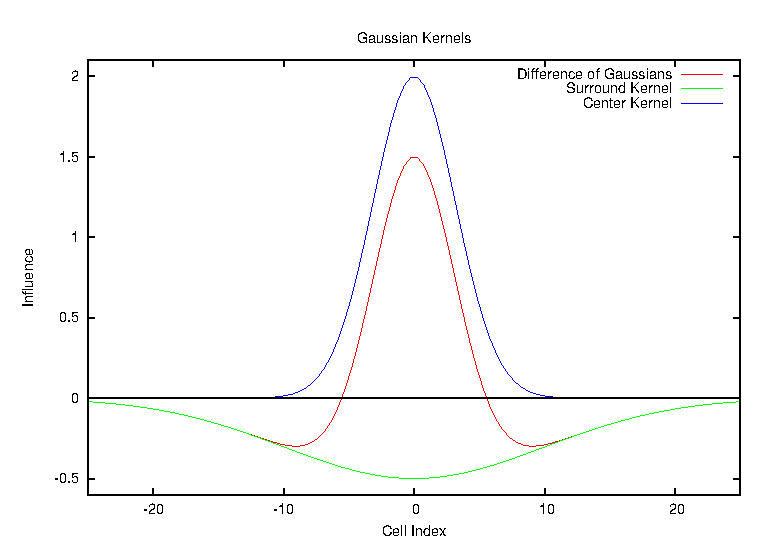
\epsfig{file=gaussians.eps,width=15cm,height=11cm}
    \caption{\label{pict1}Gaussian Kernels}
  \end{figure}
\end{center}

\vfil\eject

The plot below shows the decay rate for an exponential function; the $A$ term in the shunting equation will result in a decay term in the solved differential equation. 

\begin{center}
  \begin{figure}[h!]
    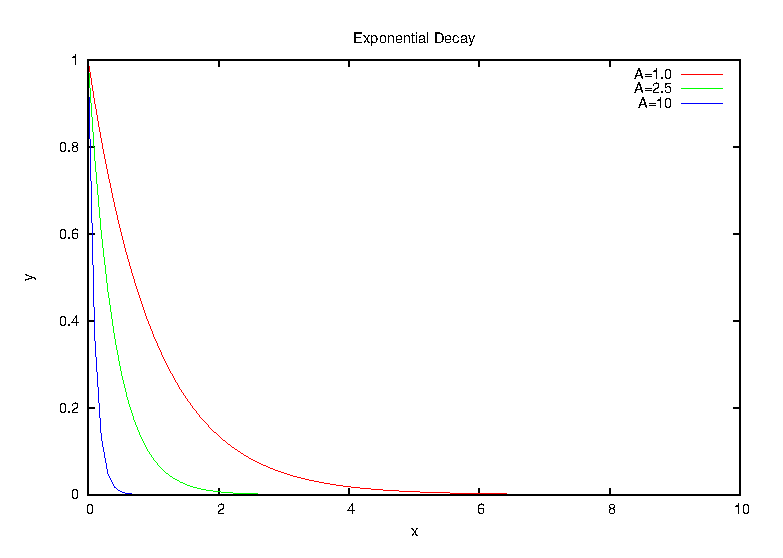
\epsfig{file=expDecay.eps,width=15cm,height=11cm}
    \caption{\label{pict1}Exponential Decay}
  \end{figure}
\end{center}

We now have what we need to generate apparent motion. Here are the criteria; given two stimuli presented one after another, our model will observe apparent motion if the space between activated sites maintains a positive response throughout the period of SOA. In other words, if the cells in the neigboring region of a stimuli can keep up their positive response until the second stimuli arrives, and if this stimuli's positive response ``overlaps'' with the previous, then there will be apparent motion. 
\vfil\eject

In order to make this occur, we could do the following: we could spread out our DoG kernel far enough so that many neighbors are encompassed by the excitatory kernel. This can be done by changing the standard deviation term $\mu$ in the excitatory kernel to a smaller value. The $\nu$ value in the inhibitory kernel should be changed proportionally to maintain center-surround, and the peak values $C$ and $E$ should be correct in any situation (ideally $C>E$). The number of neighbors we'd like to encompass depends on how far apart the stimuli are; if the stimuli are 10 neighbors apart, then the excitatory kernel should cover at least 10 neighbors. 

\begin{center}
  \begin{figure}[h!]
    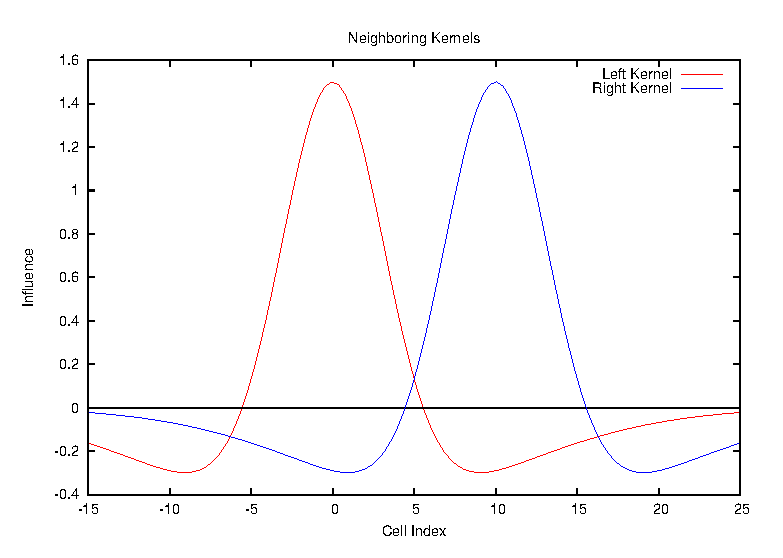
\epsfig{file=neighborGaussians.eps,width=15cm,height=11cm}
    \caption{\label{pict1}Overlapping Gaussian Kernels}
  \end{figure}
\end{center}

\vfil\eject

Furthermore, the excitatory response of the first stimuli should persist long enough to be absorbed into the excitatory response of the next stimuli. In the example of the 10 neighbors, this would only work if the two stimuli were presented  almost at the same time. Because the response decays depending on how we set the $A$ term, we must also take that into account. Larger $A$ values mean the stimuli must be closer together in both distance and time. 

\begin{center}
  \begin{figure}[h!]
    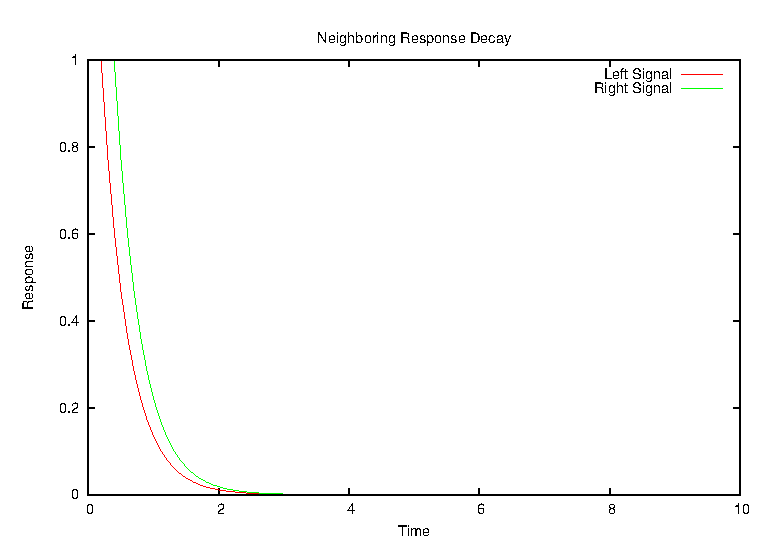
\epsfig{file=neighborDecay.eps,width=15cm,height=11cm}
    \caption{\label{pict1}Overlapping Exponential Decays}
  \end{figure}
\end{center}

\vfil\eject

\begin{center}
  \begin{figure}[h!]
    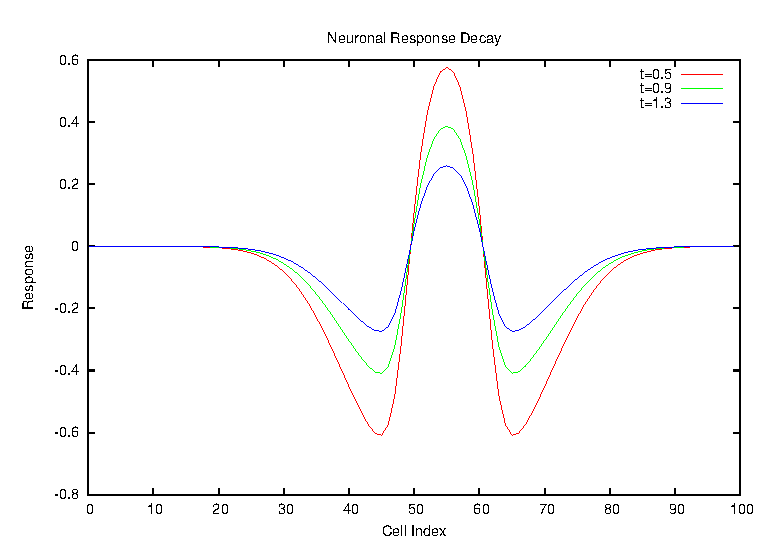
\epsfig{file=decay.eps,width=15cm,height=11cm}
    \caption{\label{pict1}Gaussian Response decaying with time}
  \end{figure}
\end{center}

Note that the response profile decays exponentially, meaning the next overlapping response must arrive before it decays toomuch. 

\vfil\eject

{\bf Results}

I achieved apparent motion with the following parameters: $A=1,B=1,C=2,D=1,E=0.5,\mu=0.05,\nu=0.005,m=0.5,$SOA$=1.5,k=55,l=65,n=100$. 
\smallskip

Below is the network response to the first stimulus.
\begin{center}
  \begin{figure}[h!]
    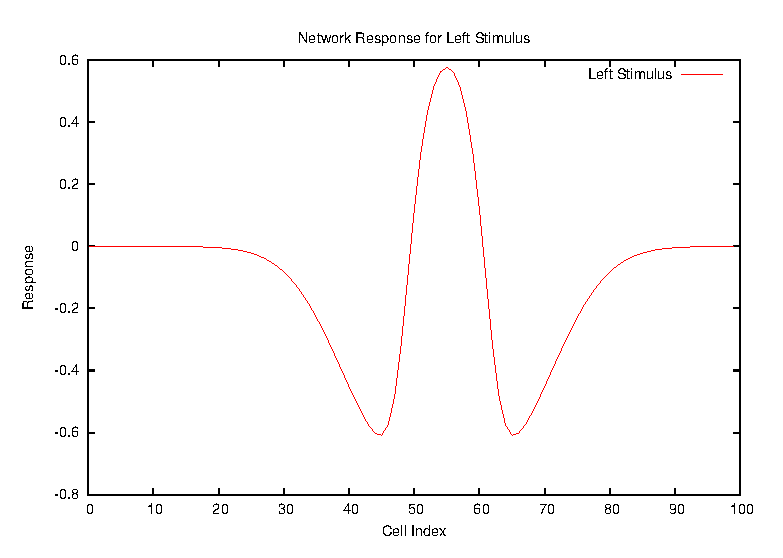
\epsfig{file=leftOnly.eps,width=15cm,height=11cm}
    \caption{\label{pict1}Left Stimulus}
  \end{figure}
\end{center}

\vfil\eject

Here is the network response to the second stimulus. 

\begin{center}
  \begin{figure}[h!]
    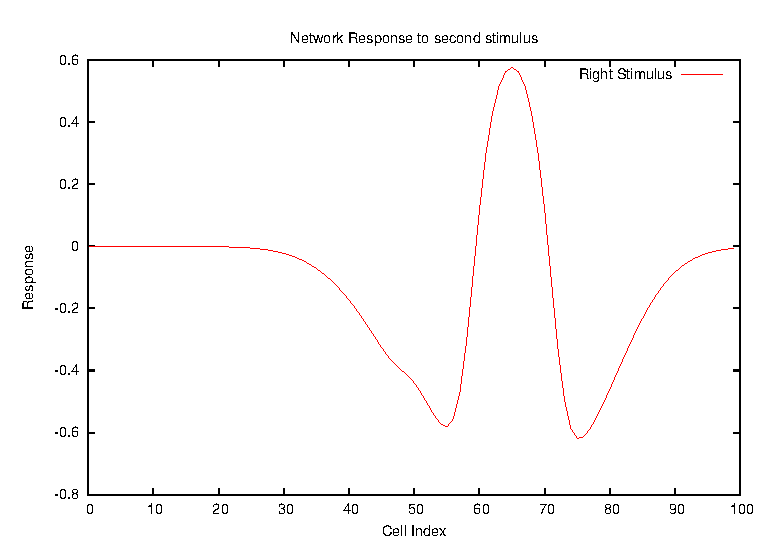
\epsfig{file=rightOnly.eps,width=15cm,height=11cm}
    \caption{\label{pict1}Right Stimulus}
  \end{figure}
\end{center}

\vfil\eject

The traveling waves occured in between the previous two plots

\begin{center}
  \begin{figure}[h!]
    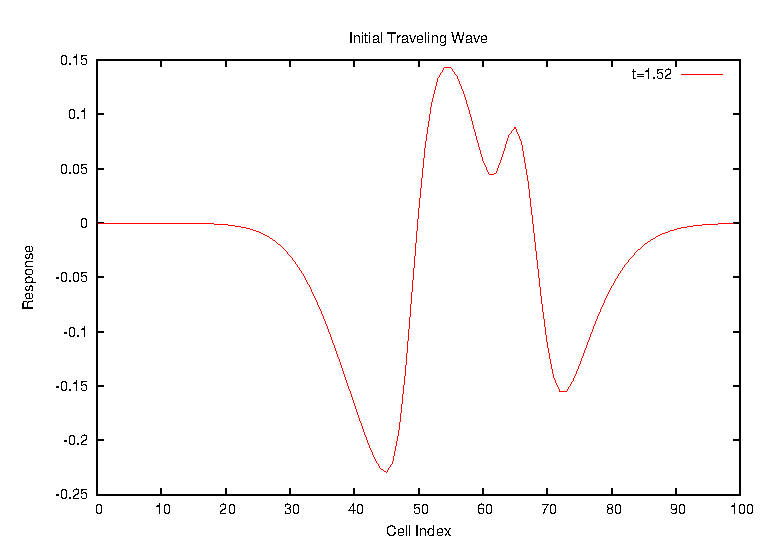
\epsfig{file=travel1.eps,width=4cm,height=4cm}
    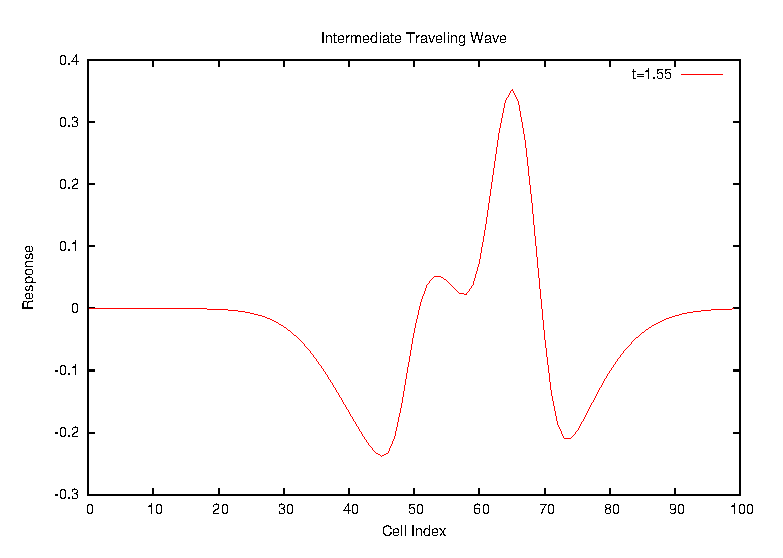
\epsfig{file=travel2.eps,width=4cm,height=4cm}
    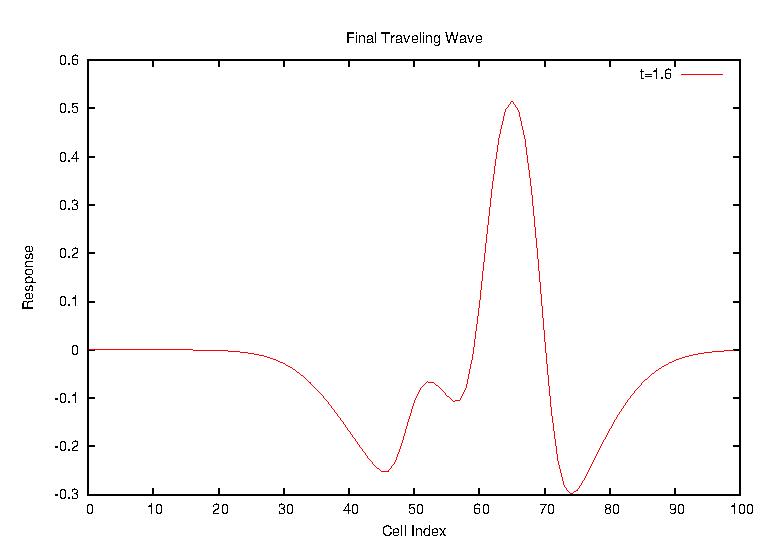
\epsfig{file=travel3.eps,width=4cm,height=4cm}
    \caption{\label{pict1}Traveling Waves}
  \end{figure}
\end{center}

{\bf Conclusion}
\smallskip

Compared with my network in assignment two, this network varies in several ways. Namely the decay rate is much slower and kernels are much wider. In terms of realism, the veracity of such a network depends on your sense of scale. For my 100 neurons, I deemed a length of $10$ neighbors between activation sites sufficient for apparent motion. In order to make this work I had to spread my kernels out enough to cover these 10 and slow my decay enough to make the positive response persist.
\smallskip

The persisting bump in the response between sites is called a travelling wave because it appears to roll between the first and second stimuli. Depending on the application of such a network this may or may not be sufficient. A distance of 10 seemed like a big enough distance for me to actually see a travelling wave, but in actuality 10 neurons may be much too large of a distance. Ideally I'd have some psychophysical data to replicate based on real subject, but I haven't studied enough to use such data. 
\smallskip

The bottom line is that depending on what your scale is, apparent motion can be achieved in a number of ways. Realistic decay rates, delays between stimuli, and distances between stimuli depend on how you want to use the model, but using the techniques outlined here a number of situations could exhibit the phenomenon. 

\end{document}
